\section{Introduction}
\begin{frame}
    \frametitle{NP Problems and the Knapsack Problem}

    \begin{columns}[T] % Use columns for better side-by-side layout
        % Left Column: Complexity Diagram
        \begin{column}{0.5\textwidth}
            \begin{figure}
                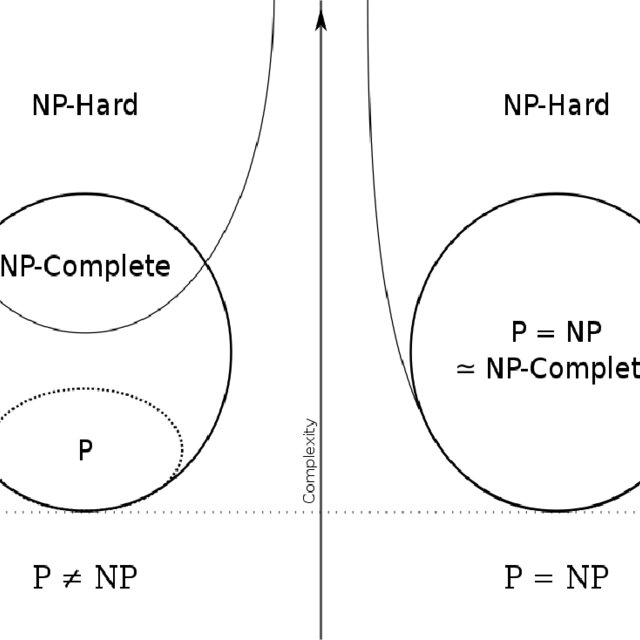
\includegraphics[width=\textwidth, height=0.75\textheight]{np-venn}
                \caption{Landscapes of computational complexity.}
                \label{fig:np-venn}
            \end{figure}
        \end{column}
        
        % Right Column: Problem Definition
        \begin{column}{0.5\textwidth}
            \textbf{Knapsack Problem Description:}
            \begin{itemize}
                \item Given $n$ items and a knapsack with capacity $W$.
                \item Each item $i$ has a weight $w_i$ and a value $v_i$.
            \end{itemize}
            
            \vspace{0.5em}
            
            \textbf{Objective:}
            \begin{itemize}
                \item Maximize the total value of selected items, subject to the total weight not exceeding $W$.
                \item Each item must either be taken (1) or left (0).
            \end{itemize}
            
            \vspace{0.5em}
            
            \textbf{Mathematical Formulation:}
            \begin{align*}
                \text{maximize} \quad & \sum_{i=1}^{n} v_i x_i \\
                \text{subject to} \quad & \sum_{i=1}^{n} w_i x_i \le W \\
                & x_i \in \{0, 1\}, \quad \forall i
            \end{align*}
        \end{column}

    \end{columns}
\end{frame}